\chapter{Εργαλεία}
\label{chapter:tools}

Στο κεφάλαιο αυτό παρουσιάζονται τα βασικά εργαλεία που
χρησιμοποιήθηκαν σε όλη τη διάρκεια της παρούσας διπλωματικής εργασίας. Συγκεκριμένα, παρουσιάζεται το μεσολειτουργικό σύστημα ROS στο οποίο βασίστηκαν οι υλοποιήσεις των συστημάτων και τα πειράματα, το Gazebo στο οποίο πραγματοποιήθηκαν οι προσομοιώσεις των πειραμάτων, το Rviz με το οποίο οπτικοποιούνται τα δεδομένα κατά την εκτέλεση των αλγορίθων. Στη συνέχεια, παρουσιάζεται το Navigation Stack, που αποτελεί τη δομή η οποία συντονίζει την πλοήγηση του οχήματος στον χώρο. Τέλος, γίνεται μια σύντομη αναφορά στις γλώσσες προγραμματισμού που επιλέχθηκαν κατά την υλοποίηση των αλγορίθμων.

\section{Robot Operating System (ROS)}
\label{section}

To Robot Operating System \cite{ros2009} αποτελεί το πιο διαδεδομένο σύστημα υλοποίησης ρομποτικών συστημάτων. Αποτελεί ένα μεσολειτουργικό (middleware) σύστημα, το οποίο διασυνδέει το λογισμικό (software) με το υλικό (hardware) με έναν τέτοιο τρόπο που η δημιουργία ρομποτικών συστημάτων και εφαρμογών είναι πιο απλή και γρήγορη. Περιλαμβάνει πολλά χαρακτηριστικά των λειτουργικών συστημάτων, όπως ο χαμηλού επιπέδου έλεγχος των συσκευών, η δημιουργία πλήθους διεργασιών και η παραλληλοποίηση των συστημάτων, η μετάδοση μηνυμάτων μεταξύ των διεργασιών αυτών, η διαχείρηση πακέτων. Επίσης, παρέχει χρήσιμα εργαλεία και βιβλιοθήκες για την ολοκληρωτική διαχείρηση κώδικα από πολλαπλούς υπολογιστές. 

Το ROS είναι μια πλατφόρμα ανοικτού κώδικα που έχει ως κύριο στόχο την απλοποίηση της διαδικασίας δημιουργίας ρομποτικών εφαρμογών. Η δόμηση της είναι τέτοια που εξυπηρετεί αυτό στον σκοπό. Συγκεκριμένα, ο κώδικας μπορεί και είναι επαναχρησιμοποιήσιμος, καθώς η κάθε εφαρμογή αποτελείται από ένα πλήθος κατανεμημένων διεργασιών (Nodes) που δίνει την δυνατότητα ανεξάρτητης ανάπτυξης των διαφόρων διεργασιών. Οι διεργασίες ομαδοποιούνται σε πακέτα (Packages) και στοίβες (Stacks), ώστε να είναι εύκολη η διανομή και ο έλεγχος τους μεταξύ των ερευνητών. Τέλος, μόνο κατά την συνολική εκτέλεση τους υπάρχει η ανάγκη συγκέντρωσης των διάφορων αυτών τμημάτων.

\section{Εργαλεία Προσομοίωσης}
\label{section:simulation_tools}

Το Gazebo\footnote{\href{http://gazebosim.org/}{http://gazebosim.org/}} αποτελεί ένα περιβάλλον προσομοίωσης ρομποτικών εφαρμογών σε τρισδιάστατα εικονικά περιβάλλοντα. Περιλαμβάνει όλους τους φυσικούς νόμους ενός πραγματικού περιβάλλοντος, κάτι που έχει ως αποτέλεσμα την προσομοίωση πραγματικών πειραμάτων σε ρεαλιστικές συνθήκες με μικρά σφάλματα σε σχέση με τα αντίστοιχα πραγματικά πειράματα. Επιπλέον, περιλαμβάνει ένα μεγάλο σύνολο από διαθέσιμα ρομπότ, αισθητήρες και περιβάλλοντα, κάνοντας πιο εύκολη την υλοποίηση των πειραμάτων.

Το ρομποτικό όχημα που χρησιμοποιείται στην εργασία αυτή είναι το turtlebot2\footnote{\href{https://www.turtlebot.com/turtlebot2/}{https://www.turtlebot.com/turtlebot2/}} το οποίο είναι προμηθευμένο με ένα LiDAR τοποθετημένο στο πάνω μέρος του για την ασφαλή κίνηση και την ακριβή εκτίμηση της θέσης του στον χώρο.

Επίσης, σημειώνεται το ROS έχει την υποδομή της άμεσης σύνδεσης των υπολοίπων συστημάτων με το Gazebo, καλώντας το κατά την εκκίνηση του συνόλου των διεργασιών. Μάλιστα, το Gazebo λειτουργεί ως μια ανεξάρτητη διεργασία, η οποία επικοινωνεί συνεχώς με όλες τις υπόλοιπες. 

Το ROS visualiziation ή Rviz\footnote{\href{http://wiki.ros.org/rviz}{http://wiki.ros.org/rviz}} χρησιμοποιείται για την τρισδιάστατη οπτικοποίηση όλων των δεδεμένων του συστήματος το οποίο τρέχει στον υπολογιστή. Αυτά τα δεδομένα μπορεί να αφορούν μετρήσεις από διάφορους αισθητήρες, πληροφορίες κατάστασης του ρομπότ και του περιβάλλοντα χώρου, ένα εικονικό μοντέλο του ρομπότ κ.α. Επίσης, μπορεί να παρουσιάσει πληροφορίες που προκύπτουν από τις διεργασίες που υλοποιούνται, όπως για παράδειγμα την επισήμανση του σημείου στόχου κατά την πλοήγηση του ρομπότ σε έναν χώρο.


\section{Navigation Stack}
\label{section:navigation_stack}

Η πλοήγηση του ρομποτικού οχήματος υλοποιήθηκε με τη χρήση ενός stack πακέτων που προσφέρει το ROS, του navigation\footnote{\href{http://wiki.ros.org/navigation}{http://wiki.ros.org/navigation}}. Αυτό περιέχει ένα σύνολο πακέτων τα οποία χρησιμοποιούν τα δεδομένα της οδομετρίας, των αισθητήρων και του χάρτη του χώρου. Δηλώνοντας ένα σημείο ως στόχο της πλοήγησης δημιουργεί το κατάλληλο σύνολο εντολών ταχύτητας τις οποίες πρέπει να ακολουθήσει το όχημα για να κατευθυνθεί στον στόχο αυτό, χωρίς να συγκρούεται με εμπόδια του περιβάλλοντα χώρου. Η συνολική δομή του stack παρουσιάζεται στο \autoref{fig:navigation_stack_overview}.

\begin{figure}
    \centering
    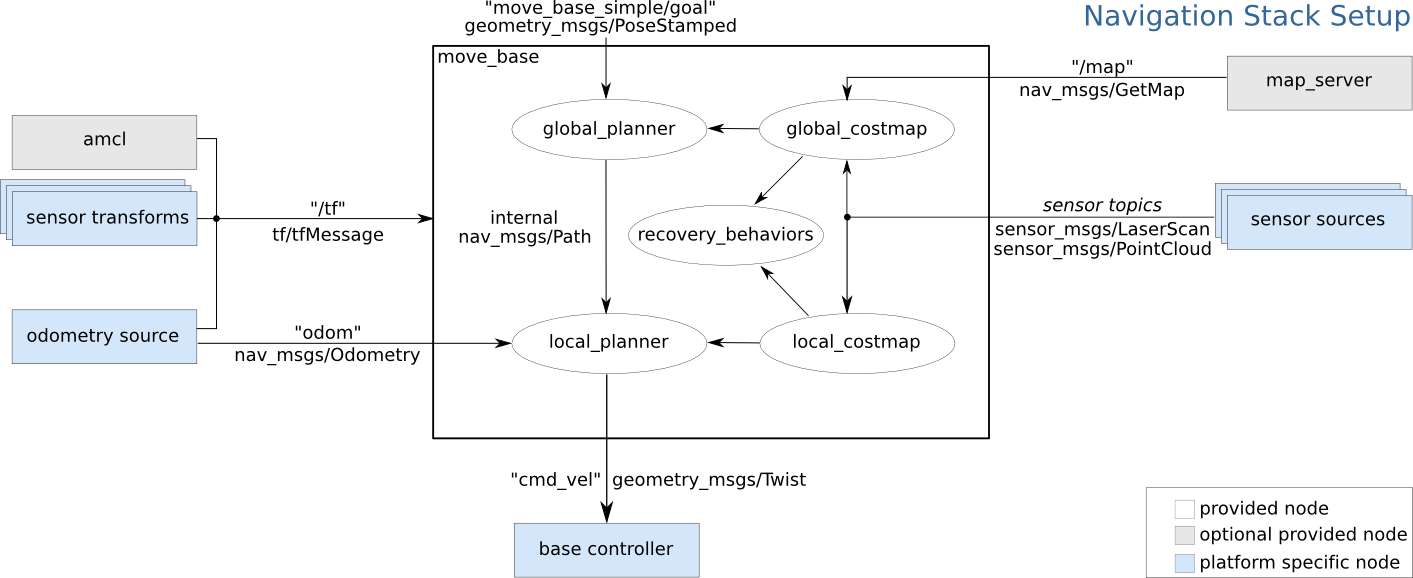
\includegraphics[width=\textwidth]{./images/chapter4/overview_nav_stack.png}
    \caption{Δομή Navigation Stack}
    Πηγή: \href{http://wiki.ros.org/navigation/Tutorials/RobotSetup}{http://wiki.ros.org/navigation/Tutorials/RobotSetup}
    \label{fig:navigation_stack_overview}
\end{figure}

Υπάρχουν, λοιπόν, δύο διαφορετικοί σχεδιαστές μονοπατιών, ο τοπικός (local planner) και ο καθολικός (global planner). Και οι δύο διαβάζουν την τρέχουσα θέση του οχήματος από τη διεργασία amcl και τον χάρτη του χώρου από την διεργασία map\_server και προσπαθούν να δημιουργήσουν μια ασφαλή πορεία μέχρι το σημείο στόχο. Ο global planner δημιουργεί ένα συνολικό μονοπάτι (global path) από την τρέχουσα θέση μέχρι τον στόχο, χωρίς να δίνει ιδιαίτερη έμφαση σε λεπτομερείς κινήσεις και μικρά εμπόδια στο περιβάλλον. Αντίθετα, ο local planner δημιουργεί ένα μονοπάτι με μικρή συνολική απόσταση (local path) που προσπαθεί να προσεγγίσει το global path ελέγχοντας με μεγαλύτερη ακρίβεια για κοντινά εμπόδια και δυναμικές αλλαγές του περιβάλλοντος προσαρμόζοντας τις κινήσεις του οχήματος. Στην εργασία αυτή χρησιμοποιήθηκαν οι εξής:
\begin{itemize}
    \setlength\itemsep{-0.2em}
    \item teb\_local\_planner ,\footnote{\href{http://wiki.ros.org/teb_local_planner}{http://wiki.ros.org/teb_local_planner}}
    \item global\_planner\footnote{\href{http://wiki.ros.org/global_planner}{http://wiki.ros.org/global_planner}}
\end{itemize}

Για την ασφαλή μετάβαση του οχήματος μέσα στον χώρο δημιουργούνται δύο χάρτες με τιμές κόστους (costmaps) που περιέχουν πληροφορίες για τα εμπόδια του χώρου. Ο ένας χάρτης χρησιμοποιείται από τον global planner και χρησιμοποιεί την δομή ολόκληρου του περιβάλλοντος για την δημιουργία του συνολικόυ μονοπατιού πλοήγησης, ενώ ο δεύτερος χρησιμοποιείται από τον local planner για τοπική αποφυγή εμποδίων.







\section{Γλώσσες Προγραμματισμού}
\label{section:software}

Οι ρομποτικές εφαρμογές που χρησιμοποιούν την υποδομή του ROS συνήθως αναπτύσσονται είτε σε Python\footnote{\href{https://www.python.org/}{https://www.python.org/}} είτε σε C++\footnote{\href{http://www.cplusplus.com/}{http://www.cplusplus.com/}}. Σε αυτή την διπλωματική χρησιμοποιήθηκε η Python, καθώς δίνει τη δυνατότητα εύκολης ανάπτυξης κώδικα και γρήγορου ελέγχου. Έχει, όμως, ένα σημαντικό μειονέκτημα. Ο χρόνος εκτέλεσης κώδικα γραμμένο σε Python είναι μεγάλος. Για τον λόγο αυτό, σε ορισμένες περιπτώσεις που η ταχύτητα εκτέλεσης είναι μείζονος σημασίας, έχουν αναπτυχθεί αλγόριθμοι σε C και έχουν εισαχθεί στον κώδικα της Python με την χρήση της βιβλιοθήκης Cffi\footnote{\href{https://cffi.readthedocs.io/en/latest/}{https://cffi.readthedocs.io/en/latest/}}. Τέλος, μια από τις πιο σημαντικές βιβλιοθήκες που χρησιμοποιείται κατά κόρον είναι η \emph{numpy}\footnote{\href{https://www.numpy.org/}{https://www.numpy.org/}} η οποία διαχειρίζεται τις μεταβλητές των προγραμμάτων και υλοποιεί γρήγορα πράξεις μεταξύ τους.




